\documentclass[11pt]{article}
\usepackage[margin=1in]{geometry}
\usepackage{graphicx,booktabs,amsmath,amssymb,hyperref,xcolor,caption,subcaption,enumitem}
\hypersetup{colorlinks=true,linkcolor=blue!50!black,citecolor=blue!50!black,urlcolor=blue!50!black}
\graphicspath{{../figures/}}
\captionsetup{font=small,labelfont=bf}
\newcommand{\eq}{\texttt{=}}

\title{A Bump and a Comb: How Llama-3.1-8B Multiplies}
\author{Mechanistic interpretability case study}
\date{November 2026}

\begin{document}
\maketitle

\begin{abstract}
We reverse-engineer how the base model Llama-3.1-8B computes products $a\times b$ of two-digit by one- or two-digit numbers whose product fits in a single token ($ab\le 999$). The model solves these problems almost perfectly (99.7\%). We show that it does so with a two-part code read out at the final \eq{} token. First, two attention heads (L15H14 and L16H21) copy operands $b$ and $a$ to the \eq{} position at layers 15--16. Then MLP neurons in layers 18--31 write the answer through two families of neurons with complementary roles. \emph{Magnitude neurons} detect the approximate size of $ab$ and write a smooth bump over the number line. \emph{Modular neurons} detect the residue of $ab$ modulo small integers (mostly 2, 4, 5, 8, 10, and partly 3) and write a periodic comb over all numbers sharing that residue. Neither family alone pins down the answer: the bump is about $\pm60$ wide, and the comb has aliases one period away. Their sum, however, peaks sharply at the true product, and the direct effects of these 494 neurons alone select the correct token for 97\% of problems. Causal interventions confirm the decomposition. Ablating modular neurons yields \emph{nearby} answers with the \emph{wrong last digit}, while ablating magnitude neurons yields \emph{far-off} answers that often keep the \emph{right last digit}. Transplanting one family's activations from another problem moves only the residue (or only the magnitude) of the answer, and transplanting both rewrites the answer to the donor's product 93\% of the time. Using only class-mean activations, we can make the model output a chosen units digit, move its answer to a chosen magnitude, and write arbitrary target numbers. Exact writes become more common as the residue information we supply gets finer (10\% $\to$ 36\%), as the mechanism predicts. The same picture explains the model's characteristic failure on 4-digit products, which errs by $\pm10$ or $\pm20$, with accuracy decaying as products grow.
\end{abstract}

\begin{figure}[t]
\centering
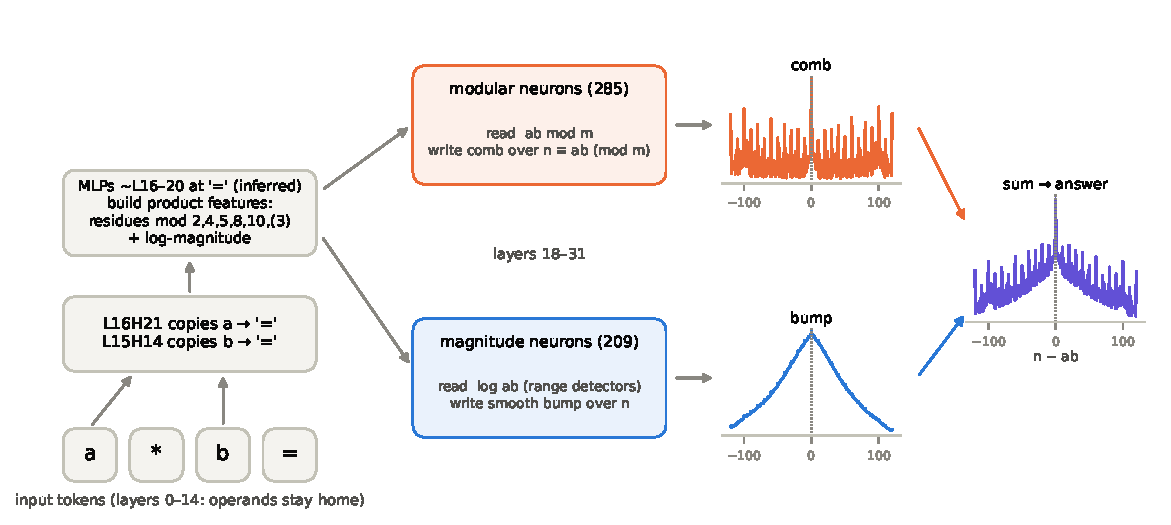
\includegraphics[width=\linewidth]{fig_schematic.pdf}
\caption{\textbf{Mechanism overview.} Operands stay at their own tokens until layers 15--16, when two heads copy them to the final \eq{} token. Product features then appear there (inferred from probes), and two neuron families in layers 18--31 write the answer. Magnitude neurons add a broad bump centered on $ab$; modular neurons add a comb that raises every number congruent to $ab$ modulo small integers. Insets show the actual mean direct logit contributions of each family, aligned on the true product (Section~\ref{sec:neurons}); their sum peaks at the answer.}
\label{fig:schematic}
\end{figure}

\section{Introduction}
Large language models perform arithmetic far beyond memorized tables, yet they do not appear to run the schoolbook algorithm. For addition, prior work found Fourier-like number features with periods 2, 5, and 10 \cite{zhou2024}, helical representations \cite{kantamneni2025}, and a ``bag of heuristics'' of neurons that each recognize patterns in the operands and promote matching result ranges or residues \cite{nikankin2024}. Multiplication is harder: the product's digits depend on carries across all operand digits, and the product spans a much larger range.

We give an end-to-end account of how Llama-3.1-8B computes single-token products. Our central finding is that the answer token is chosen by combining two imprecise but complementary signals (Figure~\ref{fig:schematic}).
\begin{itemize}[leftmargin=1.2em,itemsep=1pt]
  \item a \textbf{magnitude code} (``the answer is around 700''), which is precise to roughly 5--8\% of the product;
  \item a \textbf{residue code} (``the answer is even, a multiple of 4, ends in 4, and is not divisible by 3''), which is exact but periodic.
\end{itemize}
Each code is carried by an identifiable family of MLP neurons. A neuron's input selectivity matches its output effect: a neuron that fires when $ab\equiv0\pmod 3$ promotes all multiples of 3. Adding a bump and a comb in logit space yields a sharp peak at the true product, in the spirit of a residue number system plus a coarse magnitude estimate.

Our evidence combines four kinds of experiment:
\begin{itemize}[leftmargin=1.2em,itemsep=1pt]
  \item activation patching to locate the computation (Section~\ref{sec:locate});
  \item probes and the logit lens to time when product features appear (Section~\ref{sec:represent});
  \item neuron-level analysis of input selectivity and output patterns (Section~\ref{sec:neurons});
  \item causal interventions: double-dissociation ablations, activation transplants, and donor-free steering that writes chosen answers (Section~\ref{sec:interventions}).
\end{itemize}
Code, results, and the full research log are in the accompanying repository.

\section{Setup}
\label{sec:setup}
\paragraph{Model and prompts.} We study the base model Llama-3.1-8B in bfloat16. Unless stated otherwise, every prompt is a fixed four-shot prefix followed by the query,
\begin{center}\texttt{3*4=12\textbackslash n15*6=90\textbackslash n21*13=273\textbackslash n8*7=56\textbackslash n$a$*$b$=}\end{center}
and we read the greedy next-token prediction. The Llama-3 tokenizer encodes every integer from 0 to 999 as a single token, and longer integers in left-aligned chunks of three digits (\texttt{1081}$\to$\texttt{108},\texttt{1}).

\paragraph{Main dataset.} We use all $a\in[10,99]$, $b\in[2,99]$ with $ab\le 999$ (2210 problems). Here the query is exactly four tokens (\texttt{$a$}, \texttt{*}, \texttt{$b$}, \eq{}), and the model must emit the whole product as one token out of the 1000 number tokens. ``The answer position'' always means the final \eq{} token. When we read predictions under interventions, we take the argmax over the 1000 number tokens.

\paragraph{Direct logit attribution.} For an MLP neuron with activation $h$ (the input to \texttt{down\_proj}) and output weight $w$, its direct effect on the logit of number token $n$ is $h\cdot(\tilde W_U[n]\cdot w)/\sigma$. Here $\tilde W_U$ is the unembedding with the final RMSNorm gain folded in and centered over the 1000 number tokens, and $\sigma$ is the final residual RMS. We call the vector $(\tilde W_U[n]\cdot w)_{n=0}^{999}$ the neuron's \emph{output pattern}.

\section{Behavior}
\label{sec:behavior}
Over all $a,b\in[1,99]$ the model is 100\% accurate on 1-digit$\times$1-digit and 2-digit$\times$1-digit problems and 79.4\% on 2-digit$\times$2-digit problems. Accuracy splits sharply on whether the product fits in one token: 99.7\% for $ab<1000$ versus 74.9\% for 4-digit products (Figure~\ref{fig:behavior}a). The 4-digit errors have a telling signature (Figure~\ref{fig:behavior}b):
\begin{itemize}[leftmargin=1.2em,itemsep=1pt]
  \item the predicted length is almost always right (99.9\%);
  \item the last digit is right 90\% of the time;
  \item the error is usually exactly $\pm10$ or $\pm20$ (median $|\text{error}|=10$).
\end{itemize}
In other words, the model knows roughly how big the product is and what it ends in, but misses the tens digit. Accuracy on 4-digit products also falls steadily with size, from 90\% for products in $[1000,2000)$ to 50\% in $[8000,9000)$. Single-token products show no such decline (99.2--100\% in every range). Section~\ref{sec:discussion} explains both patterns.

\begin{figure}[t]
\centering
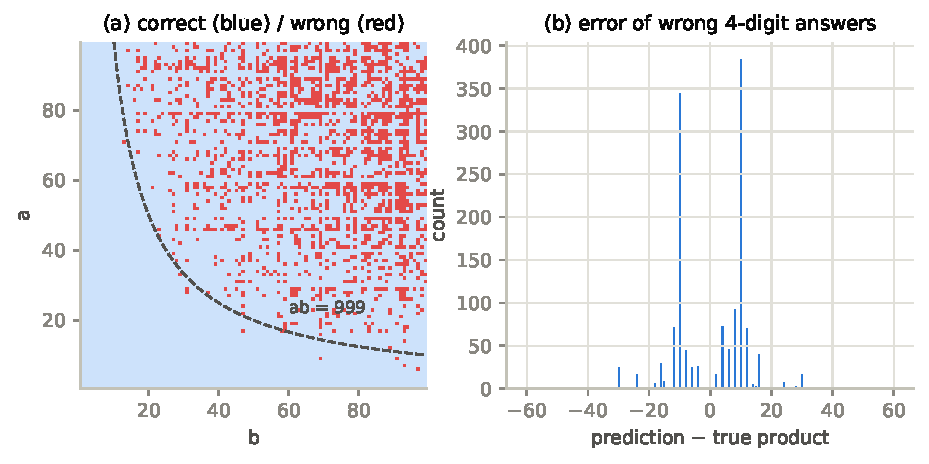
\includegraphics[width=0.92\linewidth]{fig_behavior.pdf}
\caption{\textbf{Behavior.} (a) Greedy correctness for $a,b\in[1,99]$. Errors appear almost only above the $ab=999$ curve, where the product needs two tokens. (b) Prediction minus truth for wrong 4-digit answers: errors concentrate on $\pm10$ and $\pm20$.}
\label{fig:behavior}
\end{figure}

\section{Where the computation happens}
\label{sec:locate}
\paragraph{Residual patching.} We corrupt one operand, replacing it with a different number of the same digit length that also gives a single-token product, and restore the clean residual stream at one (layer, position). We measure the recovered fraction of the clean-minus-corrupt logit difference ($n=120$ pairs per operand). Information about $a$ lives only at the $a$ token through layer 14 (recovery $\approx1.0$). It moves to \eq{} between layers 15 and 17: at layer 16, patching the $a$ position recovers only 0.17 and patching \eq{} recovers 0.79. From layer 18 on it is entirely at \eq{} (Figure~\ref{fig:patching}a,b); operand $b$ behaves the same way. The \texttt{*} and newline tokens carry nothing.

\paragraph{Component patching.} We corrupt both operands and patch single components at \eq{} ($n=200$). Attention matters only at layers 15 (0.38) and 16 (0.29), while MLPs contribute at every layer from 15 to 31, each recovering 0.07--0.33 (Figure~\ref{fig:patching}c). At the head level, two heads dominate: L15H14 (0.22) and L16H21 (0.20); no other head exceeds 0.05. Their attention patterns are clean. From \eq{}, L15H14 puts 96\% of its attention on $b$, and L16H21 puts 95\% on $a$. A third head, L15H15, also attends to $b$ (85\%). These heads are partially redundant: mean-ablating both at \eq{} lowers accuracy only from 99.7\% to 97.3\% (two random heads: 99.7\%).

\begin{figure}[t]
\centering
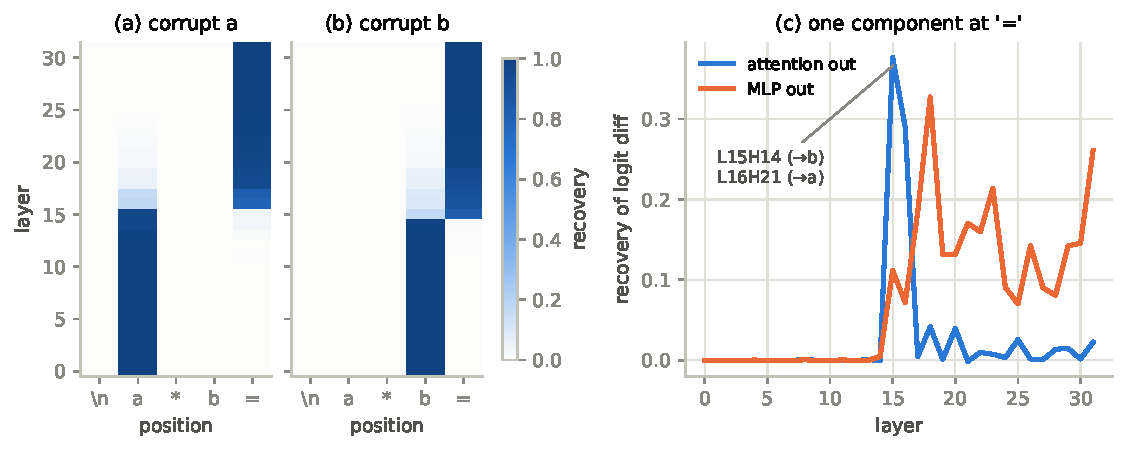
\includegraphics[width=\linewidth]{fig_patching.pdf}
\caption{\textbf{Localization.} (a,b) Residual-stream patching after corrupting operand $a$ or $b$. Operand information stays at its own token until layer $\sim$15, then moves to \eq{}. (c) Patching single attention or MLP outputs at \eq{}. Attention matters only at L15--16 (heads L15H14$\to b$ and L16H21$\to a$); the answer is then built by MLPs across L15--31.}
\label{fig:patching}
\end{figure}

\section{What is represented at the answer position}
\label{sec:represent}
We cache the residual stream at \eq{} for all 2210 problems and fit linear probes (PCA to 256 dimensions, then logistic regression; 70/30 split) at every layer.
\begin{itemize}[leftmargin=1.2em,itemsep=1pt]
  \item \textbf{Additive targets are uninformative.} Targets that are additive in the operands, such as each operand's units digit and $\log ab=\log a+\log b$, are perfectly decodable from layer 1 onward, because \eq{} carries some operand identity early. Since patching showed this early copy is not used, these probes tell us nothing about computation.
  \item \textbf{Product digits are informative.} The product's units digit is not a linear function of operand identity. Its probe sits at $\sim$0.55 through layer 16, then rises at layers 17--19 to 0.93. The hundreds digit rises over L18--20, and the \textbf{tens digit last}, over L21--24 (Figure~\ref{fig:probes}a).
  \item \textbf{Logit lens.} The exact answer becomes the top number token only late: 1\% of problems at L18, 40\% at L23, 96\% at L29 (Figure~\ref{fig:probes}b).
\end{itemize}
The ordering is the first hint of the mechanism. Residue information (the units digit) and coarse magnitude (the hundreds digit) appear first, and the tens digit, which needs both to be combined precisely, appears last.

\begin{figure}[t]
\centering
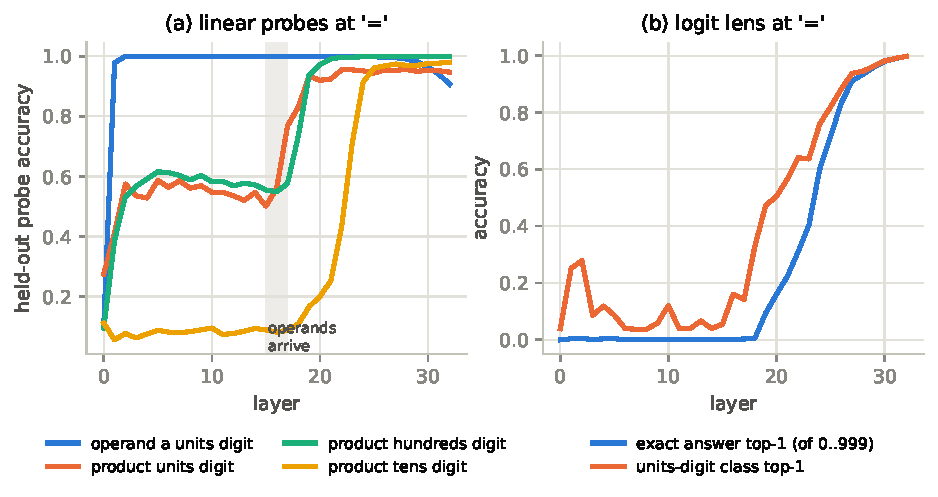
\includegraphics[width=0.95\linewidth]{fig_probes.pdf}
\caption{\textbf{Timing.} (a) Linear probes at \eq{}. Operand digits are decodable early but unused. The product's units and hundreds digits appear right after the operands arrive (L17--20); the tens digit appears last (L21--24). (b) Logit lens: the exact answer becomes top-1 between L19 and L29.}
\label{fig:probes}
\end{figure}

\section{The neurons that write the answer}
\label{sec:neurons}
\paragraph{Finding the writers.} We compute each neuron's mean direct logit attribution (DLA) to the correct answer over all problems, for every MLP neuron in layers 14--31 at \eq{}, and keep the top 60 per layer (1080 neurons). Direct effects are negligible before layer 18 and grow with depth. They are spread thin: the largest single neuron contributes 0.27 logits on average, so no single neuron is responsible for the answer.

\paragraph{Two families.} We classify each neuron by the shape of its output pattern over $n\in[0,999]$.
\begin{itemize}[leftmargin=1.2em,itemsep=1pt]
  \item \emph{Magnitude}: more than half of its variance is in the 10 lowest Fourier frequencies (periods $\ge100$).
  \item \emph{Modular, mod $m$}: the smallest $m\in\{2,\dots,100\}$ such that $n \bmod m$ explains most of the variance (above a chance-corrected 0.3). We use the smallest qualifying modulus so that, for example, mod~100 does not absorb mod~10.
\end{itemize}
Among the 200 highest-DLA neurons, 74 are magnitude neurons (total DLA 2.75 logits) and 72 are modular (about 2.3 logits). The moduli are dominated by 10, 100, 5, and 2, with fewer neurons for 3, 8, 4, 7, 11, and 20. The remaining 54 do not fit either class.

\paragraph{Input selectivity matches output pattern.} Crucially, what a neuron \emph{reads} matches what it \emph{writes}.
\begin{itemize}[leftmargin=1.2em,itemsep=1pt]
  \item \textbf{Modular neurons.} Activation is explained by the product's residue modulo \emph{the same} $m$ (mean $R^2=0.54$) and hardly at all by magnitude (0.07).
  \item \textbf{Magnitude neurons.} The reverse holds: magnitude bins explain 0.63 of the activation variance, residues 0.04.
\end{itemize}
Figure~\ref{fig:neurons} shows examples. L31N10258 is a range detector that fires for $ab\gtrsim600$ and promotes large numbers. L30N13826 (the top neuron overall) fires negatively when $3\mid ab$ and, through a negative output weight, promotes all multiples of 3. L29N1647 does the same for multiples of 8, with a weaker response at residue 4. L26N8382 handles 7. About 30\% of modular neurons are pure \emph{divisibility detectors} (the indicator $[m\mid ab]$ explains $\ge$80\% of their residue-driven variance), and they carry half of the modular DLA. The rest, mostly mod-10 neurons, respond to particular nonzero residues. For 84\% of modular neurons, the residue that drives the neuron is the residue whose logits it raises.

\begin{figure}[t]
\centering
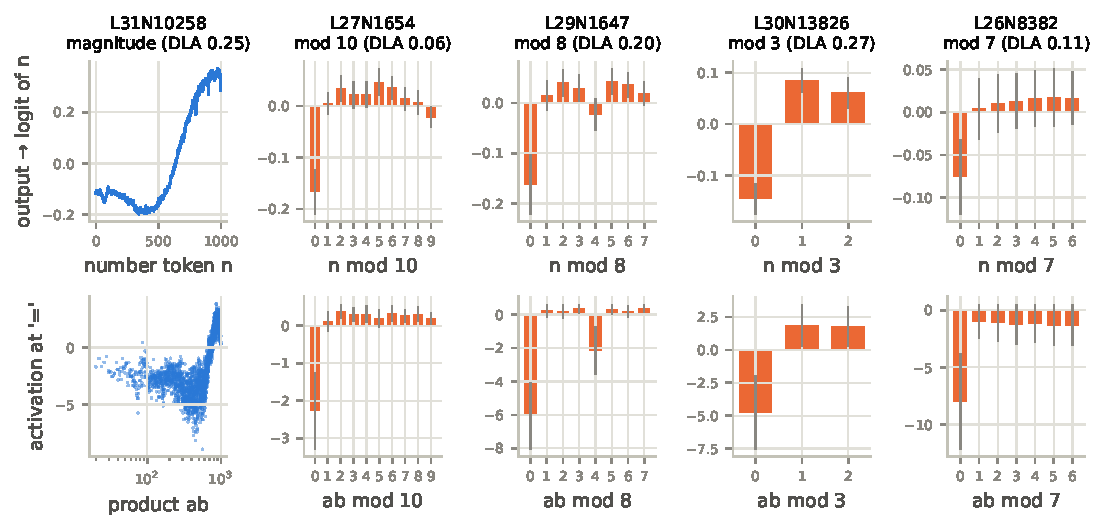
\includegraphics[width=\linewidth]{fig_neurons.pdf}
\caption{\textbf{Example neurons.} Top: output pattern (effect on the logit of number $n$ per unit activation). Bottom: activation at \eq{} across all 2210 problems. Left: a magnitude neuron (a range detector). Others: modular neurons whose activation depends on $ab \bmod m$ and whose output depends on $n \bmod m$, with matching residues. Error bars show standard deviations within each residue class.}
\label{fig:neurons}
\end{figure}

\paragraph{Bump plus comb.} To see how the families combine, we sum each family's centered direct contributions to the logits (activation minus its mean, times the output pattern) and align them on the true product (Figure~\ref{fig:groupdecomp}).
\begin{itemize}[leftmargin=1.2em,itemsep=1pt]
  \item \textbf{Magnitude neurons (209)} produce a broad tent centered on $ab$ with a half-width of about 60. Alone, its argmax is exactly right for 15\% of problems but within $\pm10$ for 79\%.
  \item \textbf{Modular neurons (285)} produce a comb: spikes at offsets that are multiples of 10, taller at $\pm20$, $\pm60$, $\pm100$, $\pm120$ (common multiples of the moduli), and tallest at 0. Alone, the comb gets the units digit right for 95\% of problems but the exact answer for only 67\%, losing the rest to aliases one period away.
  \item \textbf{Their sum} peaks sharply at the true product, and its argmax is correct for \textbf{97\%} of problems.
\end{itemize}
These 494 neurons' direct effects are therefore nearly sufficient to explain the model's choice.

\begin{figure}[t]
\centering
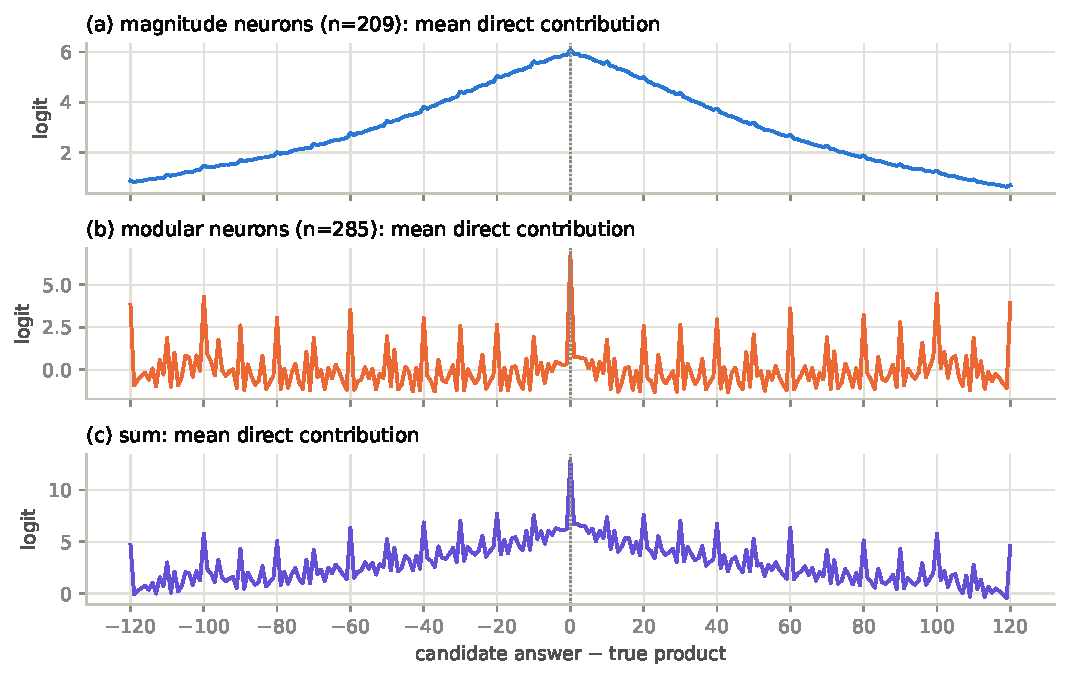
\includegraphics[width=0.92\linewidth]{fig_group_decomp.pdf}
\caption{\textbf{Bump plus comb.} Mean direct logit contribution of each neuron family to candidate answers, aligned on the true product. (a) Magnitude neurons: a broad bump. (b) Modular neurons: a comb over numbers that share the product's residues. (c) The sum peaks at the answer.}
\label{fig:groupdecomp}
\end{figure}

\section{Causal interventions}
\label{sec:interventions}
All interventions overwrite the activations of a neuron family at the \eq{} position only and leave everything else untouched. Controls use size-matched sets of random neurons from the same layers.

\paragraph{Double dissociation by ablation.} Mean-ablating either family costs about a quarter of the accuracy, but the two produce \emph{opposite kinds of errors} (Figure~\ref{fig:interventions}a). Random controls leave accuracy at 99.8\%.
\begin{itemize}[leftmargin=1.2em,itemsep=1pt]
  \item \textbf{Ablating modular neurons} leaves 73.0\% correct. Of the wrong answers, 87\% are within $\pm10$ of the truth but only 2.3\% have the right units digit. The model still knows the size but loses the residue.
  \item \textbf{Ablating magnitude neurons} leaves 71.8\% correct. Only 0.2\% of the wrong answers are within $\pm10$, yet 56\% still have the right units digit. The model keeps the residue but loses the size.
\end{itemize}

\paragraph{Activation transplants.} For each problem $x$ we pick a donor problem $y$ whose product differs by at least 100 and ends in a different digit. We then replace one family's activations at \eq{} with their values on $y$.
\begin{itemize}[leftmargin=1.2em,itemsep=1pt]
  \item \textbf{Modular transplant.} The output takes $y$'s units digit 62\% of the time (random control: 0.1\%) while staying a median of 4 away from $x$'s product.
  \item \textbf{Magnitude transplant.} The output moves to a median distance of 17 from $y$'s product (300 from $x$'s) and keeps $x$'s units digit 61\% of the time (Figure~\ref{fig:interventions}c).
  \item \textbf{Both transplants together} make the model output $y$'s answer \textbf{92.9\%} of the time.
\end{itemize}
Table~\ref{tab:examples} shows typical cases. When $16\times44$ receives donor activations from $78\times4=312$, the modular transplant yields 712: near 704, but ending in 2 and divisible by 8 like 312. The magnitude transplant yields 304: near 312, but with 704's last digit and divisibility by 8. Figure~\ref{fig:interventions}b checks residues beyond the last digit. Considering only cases where donor and original disagree modulo $m$, a modular transplant makes the output follow the donor's residue far above chance for $m=2$ (0.89), 4 (0.69), 5 (0.62), 8 (0.41), 10 (0.62), and, more weakly, 3 (0.46 vs.\ chance 0.33). A magnitude transplant does not (0.05--0.21). Moduli 7 and 9 remain at chance, so although mod-7 and mod-11 neurons exist, their causal weight is small.

\begin{table}[t]
\centering\small
\begin{tabular}{lcccc}
\toprule
problem $x$ & donor $y$ & modular transplant & magnitude transplant & both \\
\midrule
$16\times44=704$ & $78\times4=312$ & 712 & 304 & 312\\
$71\times9=639$ & $18\times2=36$ & 636 & 39 & 36\\
$10\times88=880$ & $19\times28=532$ & 888 & 550 & 532\\
$12\times22=264$ & $17\times8=136$ & 268 & 132 & 136\\
$36\times9=324$ & $64\times2=128$ & 328 & 126 & 128\\
$60\times12=720$ & $58\times3=174$ & 714 & 180 & 174\\
\bottomrule
\end{tabular}
\caption{\textbf{Transplant examples} (six of twelve problems drawn at random and printed; all twelve show the same pattern, see the research log). Modular transplants keep $x$'s magnitude but adopt $y$'s residues. Magnitude transplants move to $y$'s magnitude but keep residues of $x$ (e.g., 126 keeps $324\equiv0 \pmod 9$; 304 keeps 704's last digit and $\equiv 0 \pmod{8}$).}
\label{tab:examples}
\end{table}

\begin{figure}[t]
\centering
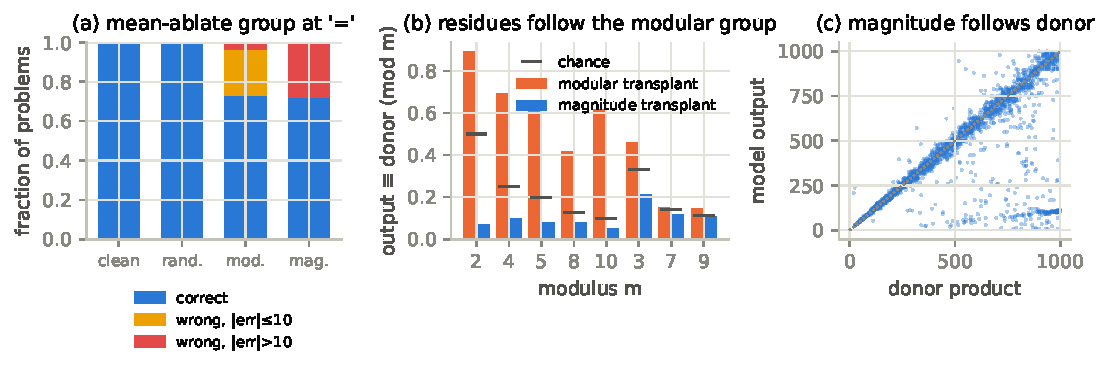
\includegraphics[width=\linewidth]{fig_interventions.pdf}
\caption{\textbf{Causal tests.} (a) Mean-ablating modular (mod.) neurons gives near-miss errors (yellow); ablating magnitude (mag.) neurons gives far-off errors (red); random (rand.) neurons do nothing. (b) After a modular transplant, the output's residue modulo $m$ follows the donor (orange) well above chance (ticks) for $m\in\{2,4,5,8,10,3\}$; after a magnitude transplant it does not (blue). (c) After a magnitude transplant, the output tracks the donor's product.}
\label{fig:interventions}
\end{figure}

\paragraph{Donor-free steering.} Transplants copy a real problem's activations. To show that we understand what the families encode, we also write answers using only \emph{class-mean} activations computed over the dataset.
\begin{itemize}[leftmargin=1.2em,itemsep=1pt]
  \item \textbf{Units-digit steering.} We set the modular neurons to their mean over all problems whose product ends in $d$. The output then ends in $d$ for 45--88\% of problems (depending on $d$; the true digit is excluded), and 90--95\% of outputs stay within $\pm10$ of the true product.
  \item \textbf{Magnitude steering.} We set the magnitude neurons to their mean over problems with $|ab-T|\le25$. The output lands near $T$ (median error 8 at $T=100$, rising to about 40 at $T=900$) and keeps its own units digit 55--78\% of the time. Because the error grows in proportion to $T$, the magnitude code has roughly constant \emph{relative} precision.
  \item \textbf{Writing arbitrary numbers.} We combine both: the modular mean for residue $t \bmod m$ and the magnitude mean for $T=t$, for random targets $t\in[100,999]$ (300 problems).
\end{itemize}
The mechanism makes a quantitative prediction about the third experiment. A comb that only fixes $t\bmod 10$, combined with a magnitude code of about $\pm20$, should get the units digit right but often miss the tens digit, and exact writes should rise as the comb carries finer residue information. That is what we observe (Table~\ref{tab:write}). Exact writes rise monotonically from 9.7\% (conditioning on $t \bmod 10$) to 36\% (conditioning on $t \bmod 120$), against a chance level of 0.1\%. The biggest jump comes when mod-3 information is added ($120=8\cdot3\cdot5$). As a control, writing the mod-120 modular mean \emph{alone} leaves the output a median of 2 from the problem's true product, so the modular class means carry no magnitude information. One caveat: finer classes average fewer problems (at least 3 each), so their means are noisier.

\begin{table}[t]
\centering\small
\begin{tabular}{lcccc}
\toprule
modular class mean conditioned on & $t \bmod 10$ & $t\bmod 20$ & $t\bmod 40$ & $t \bmod 120$\\
\midrule
output $= t$ exactly & 9.7\% & 17.0\% & 18.3\% & 36.0\%\\
units digit correct & 78.7\% & 77.0\% & 76.3\% & 82.3\%\\
median $|\text{output}-t|$ & 16 & 20 & 20 & 12\\
\bottomrule
\end{tabular}
\caption{\textbf{Writing arbitrary targets $t$} with class-mean activations (magnitude family: mean over $|ab-t|\le25$). More residue information gives more exact writes, as the bump-and-comb mechanism predicts. Chance for exact is 0.1\%.}
\label{tab:write}
\end{table}

\paragraph{Robustness to prompt format.} The neuron families were identified with the default prompt. We test them unchanged on three other formats (400 problems each), intervening at whichever position emits the number token.
\begin{itemize}[leftmargin=1.2em,itemsep=1pt]
  \item \texttt{$a$$\times$$b$=} with different few-shot examples (clean accuracy 100\%);
  \item \texttt{$a$ * $b$ =} with spaces (99.8\%);
  \item the zero-shot sentence ``The product of $a$ and $b$ is'' (99.0\%).
\end{itemize}
Transplanting both families rewrites the answer to the donor's product in 93.7\%, 92.8\%, and 77.8\% of cases respectively. The error-type dissociation replicates in the first two formats: after modular ablation, 85\% and 92\% of wrong answers are near misses with the wrong units digit, while after magnitude ablation none are. In the zero-shot sentence format, ablating modular neurons mostly produces far errors (only 10\% near). There the separation between the families is less clean, possibly because other neurons take part.

\section{Discussion}
\label{sec:discussion}
\paragraph{Why the bump-and-comb code works, and when it fails.} A single-token product only needs to be distinguished from about 1000 alternatives. A magnitude estimate accurate to roughly 5--8\% narrows the field to a few dozen candidates. Residues modulo 8, 5, and 3 then pick the right one, since numbers that agree modulo all three differ by multiples of 120. This explains why errors on single-token products are rare. It also explains the failures on 4-digit products. There, the first output token is $\lfloor ab/10\rfloor$, whose residues are not simple functions of the operands' residues. For example, its last digit is the product's tens digit, which depends on carries. The comb therefore cannot sharpen the first token. Selection must rely on a magnitude estimate whose absolute error grows with the product, which produces exactly the observed $\pm10$/$\pm20$ errors and the decline in accuracy with size. The second token (the product's units digit) is a residue and stays accurate (90\%).

\paragraph{Relation to the ``bag of heuristics'' view.} Our neurons resemble the range and modulo heuristics of \cite{nikankin2024}, and the importance of mod-2/5/10 structure echoes Fourier features found in addition \cite{zhou2024,kantamneni2025}. Our contribution is to show how these pieces form a \emph{structured} code for multiplication. Read and write residues match within each neuron, the families combine additively into a sharp peak, and the code is precise enough to be used: with class-mean activations alone we can make the model output a chosen units digit, a chosen magnitude, or a chosen number, and its success rate rises with the residue information we supply.

\section{Related work}
Mechanistic studies of arithmetic in LMs locate operand routing in attention and result computation in late MLPs \cite{stolfo2023}, in line with work showing that MLPs promote vocabulary items \cite{geva2022} and store associations that can be edited \cite{meng2022}. Fourier and modular representations appear in small transformers trained on modular arithmetic \cite{nanda2023} and in pretrained models doing addition \cite{zhou2024,kantamneni2025}. Nikankin et al.~\cite{nikankin2024} argue that Llama-3-8B solves arithmetic with a sparse set of heuristic neurons. We use the logit lens \cite{nostalgebraist2020}, activation patching, and direct logit attribution throughout.

\section{Limitations}
\begin{itemize}[leftmargin=1.2em,itemsep=1pt]
  \item \textbf{Scope.} We study single-token products ($ab\le999$, $a\ge10$) in one model. Our account of 4-digit failures is an inference from behavior and the mechanism, not a separate mechanistic analysis of the first output token.
  \item \textbf{Upstream computation.} We do not fully explain how product residues and magnitude are computed from the operands. Probes show product units digits appearing at L17--19, and MLPs at L15--20 matter under patching, but we have not traced the specific neurons that turn operand features into product residues.
  \item \textbf{Neuron selection.} Our neuron families come from the top 60 neurons per layer by direct effect. More diffuse contributions (the 54 unclassified high-DLA neurons and those outside the cache) are not characterized. The classifier thresholds are heuristic, though the causal results do not depend on fine details.
  \item \textbf{Partial effects.} Single-family ablations lower accuracy by roughly a quarter, not to zero, which points to redundancy (including via the residual stream and indirect paths). Mover-head ablations show similar redundancy.
  \item \textbf{Prompt formats.} In the zero-shot sentence format the error-type dissociation is weaker, even though transplants still work (78\%).
  \item \textbf{Unexplained failure band.} When the donor product is near 900--1000, magnitude transplants sometimes produce outputs near 100 (Figure~\ref{fig:interventions}c), possibly because leading-digit features alias between ``9xx'' and ``1xx''. We have not investigated this.
\end{itemize}

\section{Conclusion}
Llama-3.1-8B multiplies two numbers with a single-token product by copying the operands to the answer position and then combining two imprecise but complementary codes in its late MLPs: a smooth magnitude bump and a residue comb. Each is carried by a distinct, interpretable neuron family whose input selectivity matches its output effect. Ablating, transplanting, and synthesizing these codes changes the model's answers in the specific ways the mechanism predicts.

\begin{thebibliography}{9}
\bibitem{nikankin2024} Y.~Nikankin, A.~Reusch, A.~Mueller, Y.~Belinkov. Arithmetic without algorithms: Language models solve math with a bag of heuristics. \emph{arXiv:2410.21272}, 2024.
\bibitem{kantamneni2025} S.~Kantamneni, M.~Tegmark. Language models use trigonometry to do addition. \emph{arXiv:2502.00873}, 2025.
\bibitem{zhou2024} T.~Zhou, D.~Fu, V.~Sharan, R.~Jia. Pre-trained large language models use Fourier features to compute addition. \emph{NeurIPS}, 2024.
\bibitem{stolfo2023} A.~Stolfo, Y.~Belinkov, M.~Sachan. A mechanistic interpretation of arithmetic reasoning in language models using causal mediation analysis. \emph{EMNLP}, 2023.
\bibitem{meng2022} K.~Meng, D.~Bau, A.~Andonian, Y.~Belinkov. Locating and editing factual associations in GPT. \emph{NeurIPS}, 2022.
\bibitem{nanda2023} N.~Nanda, L.~Chan, T.~Lieberum, J.~Smith, J.~Steinhardt. Progress measures for grokking via mechanistic interpretability. \emph{ICLR}, 2023.
\bibitem{nostalgebraist2020} nostalgebraist. Interpreting GPT: the logit lens. \emph{LessWrong}, 2020.
\bibitem{geva2022} M.~Geva, A.~Caciularu, K.~Wang, Y.~Goldberg. Transformer feed-forward layers build predictions by promoting concepts in the vocabulary space. \emph{EMNLP}, 2022.
\end{thebibliography}
\end{document}
